%!TEX TS-program = xelatex 
%!TEX encoding = UTF-8 Unicode 

\documentclass[fontsize=11pt, paper=a4, 
DIV15,
normalheadings,
parskip=half-, 
pointlessnumbers]{scrartcl}

\usepackage[british]{babel} 

\usepackage{fontspec,xltxtra,xunicode} 
\defaultfontfeatures{Mapping=tex-text} 

\setromanfont[Mapping=tex-text]{DejaVu Serif}
\setsansfont[Scale=MatchLowercase,Mapping=tex-text]{Helvetica} 
\setmonofont[Scale=1.0]{Courier New} 

\frenchspacing

\usepackage{graphicx}
\graphicspath{{./Bilder/}}

\usepackage{longtable}

\usepackage{philokalia}

%%%

%!TEX TS-program = xelatex
%!TEX encoding = UTF-8 Unicode

\usepackage{xspace} \xspaceaddexceptions{”}
\usepackage{ifthen}

\newcommand{\ch}[1]		{chapter~\ref{#1}}
\newcommand{\sect}[1]		{section~\ref{#1}}
\newcommand{\fig}[1]		{figure~\vref{#1}}
\newcommand{\Fig}[1]		{Figure~\vref{#1}}
\newcommand{\tbl}[1]		{table~\vref{#1}}

\newcommand{\ie}			{i.e. }
\newcommand{\eg}			{e.g. }

\newcommand{\qq}			{\qquad}

\newcommand{\spitz}[1]		{\ensuremath{\langle}#1\ensuremath{\rangle}}

\newcommand{\mehrzeilen}[1][1]{\enlargethispage{#1\baselineskip}}


% Zeilenabstand

\usepackage{setspace}
\newenvironment{enum}{\begin{enumerate} \singlespacing} {\end{enumerate}}
\newenvironment{items}{\begin{itemize} \singlespacing} {\end{itemize}}


% verbatim

\usepackage{verbatim}

\usepackage{alltt}
\newcommand{\klein}{\small}
\newenvironment{exakt}[1][\small]{\singlespacing#1\begin{alltt}}{\end{alltt}}

\usepackage{shortvrb}
\MakeShortVerb{\§}


%%%%%%%%%%%%%%%%%%%%%%%%%%%%%%%%

% xml commands
% use for any xml markup, brackets supplied
\newcommand{\xml}[1]{§<#1>§}
% use for milestone tags
\newcommand{\xms}[1]{§<#1/>§}
% closing element markup
\newcommand{\xmcl}[1]{§</#1>§}
% full xml markup example
\newcommand{\xmex}[1]{§#1§}
% attribute markup, the first argument is the element name
\newcommand{\attr}[2]{§@#2§}

\newcommand{\bold}{\textbf}
% ligature
\newcommand{\li}[1]{\bold{\{}#1\bold{\}}}

\newcommand{\xs}{\scriptsize}
\newcommand{\s}{\footnotesize}

%

\newcommand{\bs}{\textbackslash}
\newcommand{\tld}{\textasciitilde}

\newcommand{\tocspace}{\addtocontents{toc}{\protect\vspace{1mm}}}

\newcommand{\unicode}[1]{{\fontspec{Apple Symbols}{\Large #1}}}
\newcommand{\§}{{\char"00A7}}

%%%%%%%%%%%%%%%%

\newcommand{\htsc}[1]{\emph{#1}}
\newcommand{\lig}[1]{\fontspec{Hoefler Text}{\Large #1}}
\newcommand{\fraktur}[1]{{\fontspec{BreitkopfFraktur}{\LARGE #1}}}

%

\newenvironment{mainrule}{}{}
\newenvironment{mainruleLessImportant}{}{}
\newenvironment{clarification}{\s}{}
\newenvironment{exception}{\htsc{Exception:}}{}
\newenvironment{note}{\textbf{Please note:}}{}
\newenvironment{crossref}{\s\ensuremath{\longrightarrow}}{}

%

\newenvironment{sampleImage}[2][]{\parbox{\linewidth}{{\htsc{Example#1}} \\[3mm] \includegraphics[width=\linewidth]{#2}}}{}
\newenvironment{sampleImageSmall}[3][]{\parbox{\linewidth}{{\htsc{Example#1}} \\[3mm] \includegraphics[#2]{#3}}}{}

\newenvironment{example}[1][]{\htsc{Example#1} \\}{}
\newenvironment{exampleTest}[2][]{\parbox{\linewidth}{\htsc{Example #1} \\[3mm] #2}}{} % ??

\newenvironment{liste}[1][]{\htsc{List#1} \\}{}
\newenvironment{tabelle}[1][]{\htsc{Table#1} \\}{}

%

\newenvironment{typeLatin}{\begin{alltt}\s\begin{tabular}{@{}l}}{\end{tabular}\end{alltt}}

\newfontfamily{\greek}[Scale=0.95]{Courier New}
\newenvironment{typeGreek}{\begin{alltt}\greek\s\begin{tabular}{@{}l}}{\end{tabular}\end{alltt}}

\newenvironment{typeMath}{\begin{alltt}\begin{tabular}{l}}{\end{tabular}\end{alltt}}

%

\newfontfamily{\muh}[Scale=0.9]{DejaVu Serif}
\newcommand{\someText}{...} % {{\muh\textit{(some text)}}}
\newcommand{\untranscribedText}{...} % {{\muh\textit{(some untranscribed text)}}}
\newcommand{\notTranscribed}{{\muh\textit{(not transcribed)}}}
\newcommand{\missingText}[1]{{\muh\textit{(#1)}}}

%% Chinese bits
\newenvironment{typeChinese}{\begin{alltt}\s\begin{tabular}{@{}l}}{\end{tabular}\end{alltt}}

\newcommand{\chin}[1]{{\fontspec{Sun-ExtA}{#1}}}
\newcommand{\sunExtA}[1]{{\fontspec{Sun-ExtA}{#1}}}
\newcommand{\sunExtB}[1]{{\fontspec{Sun-ExtB}{#1}}}

\newcommand{\mincho}[1]{{\fontspec{MS Mincho}{#1}}}
\newcommand{\hira}[1]{{\fontspec{HiraMinPro-W3}{#1}}}

\newcommand{\f}[1]{\bold{#1}} % f für fett
\newcommand{\z}[1]{\chin{#1}} % z für Zeichen


\begin{document}

\begin{center}
{\fontspec{Helvetica}{\LARGE \textbf{
Special Instructions for Euclid 1966
\\[3mm]
(Addendum to Data Entry Specs 1.1.2) 
}}} \\[5mm]
\large Wolfgang Schmidle, Klaus Thoden, Malcolm D. Hyman

\normalsize Max Planck Institute for the History of Science, Berlin, Germany

\today
\end{center}


\section{Data Entry}

Data entry should be in UTF-8, making use of the complete character repertoire found in Unicode version 5.1.0, including characters in the following blocks when applicable: 

\begin{itemize}
\item CJK Unified Ideographs Extension A (U+3499 -- U+4DFF), 
\item CJK Unified Ideographs Extension B (U+20000 -- U+2A6DF), 
\item CJK Compatibility Ideographs Supplement (U+2F800 -- U+2FA1F). 
\end{itemize}

If you experience difficulty with Chinese characters from the blocks in the supplementary plane (SMP), please let us know. We can provide assistance by providing fonts containing these characters and other technical assistance.

\section{General Markup}

The conventions for typing page breaks and numbers, running heads, headings, paragraphs, figures, and captions as specified in the standard Data Entry Specs apply,
as well as the conventions for indicating illegible characters and uncertain readings (see section 2.7.1 of the Data Entry Specs). 

\subsection{Paragraphs}

Outdented paragraphs (i.e. paragraphs where the first character is printed one space higher on the page) are marked by §<p x>§.

\begin{note}
Examples for outdented paragraphs as well as the rules in section 3 can be found in the whole-page example in \sect{section example}.
\end{note}

\section{Chinese Characters}

\subsection{Punctuation}

Type the punctuation to the right of characters.

\subsection{Spaces}

Type spaces in Chinese text as the IDEOGRAPHIC SPACE character U+3000.

\subsection{Small Characters}

Strings of small characters are marked by §<sm> </sm>§. Indicate half-column breaks by §\\§. 

\section{Whole-Page Example}
\label{section example}

This is a transcription of Euclid p. 23 (i.e. scan §0023.jpg§).

\newcommand{\chin}[1]{{\fontspec{SimSun}{#1}}}

\begin{typeLatin}
\bold{<pb><rh>}\chin{幾何原本 卷一之首}\bold{</rh>} \\
\bold{<h>}\chin{幾何原本第一卷之首}\bold{<sm>}\chin{界說三十六 求作四} \bold{\bs\bs} \chin{公論十九}\bold{</sm></h>} \\
\bold{<p>}\chin{泰西利瑪竇口譯}\bold{</p>} \\
\bold{<p>}\chin{吳凇徐光啓筆受}\bold{</p>} \\ 
\bold{<h>}\chin{界說三十六則}\bold{</h>} \\
\bold{<p>}\chin{凡造論。先當分別解說論中所用名目。故曰界說。}\bold{</p>} \\
\bold{<p>}\chin{凡歷法、地理、樂律、算章、技藝、工巧諸事。有度、有數者。皆依賴十府中。幾何府屬。凡論幾何。先從一點始。} \\
\chin{自點引之爲線。線展爲面。面積爲體。是名三度。}\bold{</p>} \\
\bold{<h>}\chin{第一界}\bold{</h>} \\
\bold{<p x>}\chin{點者、無分。}\bold{</p>} \\
\bold{<p>}\chin{無長短、廣狹、厚薄。 如下圖。}\bold{<sm>}\chin{凡圖十干爲識。干盡用十} \bold{\bs\bs} \chin{二支。支盡用八卦八音。}\bold{</sm></p>} \\
\bold{<fig>} \\
\bold{<desc>}\chin{甲}\bold{</desc>} \\
\bold{<h>}\chin{第二界}\bold{</h>} \\
\bold{<p x>}\chin{線、有長無廣。}\bold{</p>} \\
\bold{<p>}\chin{試如一平面。光照之。有光無光之間。不容一物。是線也。眞平眞圜相遇。其遇處止有一點。行則止有一 }\\
\chin{線。}\bold{</p>} \\
\end{typeLatin}



\section{Figures}
\label{section chinese figures}

\begin{mainrule}
Where a figure occurs in the text, type a §<fig>§ tag on a separate line. If you can identify a caption of the figure, mark it by §<cap> </cap>§. Additional text that describes parts of the figure is marked by §<desc> </desc>§.
\end{mainrule}

\begin{clarification}
Type the caption on a separate line after §<fig>§. A figure may have more than one description. Type each description on a separate line after §<fig>§ and §<cap>§. If the same description is repeated in a figure, type it only once.
\end{clarification}

\begin{note}
In the example in section 4, there is now an additional line §<desc>§\chin{甲}§</desc>§ after the §<fig>§ tag.
\end{note}


\begin{tabular}{@{}ll}
\parbox[b]{8.3cm}{
\htsc{Examples} \\
\begin{typeLatin}
\bold{<fig>} \\
\bold{<cap>}\chin{第九鐵餅正看圖}\bold{<sm>}\chin{四分之一}\bold{</sm>}\bold{</cap>} \\
\bold{<desc>}\chin{秋}\bold{</desc>} \\
\bold{<desc>}\chin{收}\bold{</desc>} \\
\bold{<fig>} \\
\bold{<cap>}\chin{鐵餅剖看圖}\bold{</cap>} \\
\bold{<desc>}\chin{秋}\bold{</desc>} \\
\bold{<desc>}\chin{螺帽}\bold{</desc>} \\
\bold{<desc>}\chin{收}\bold{</desc>} \\
\bold{<desc>}\chin{螺鍵}\bold{</desc>} 
\end{typeLatin}} &
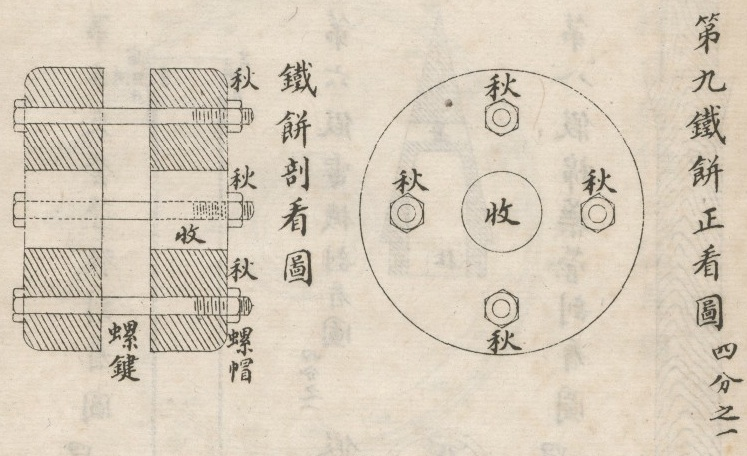
\includegraphics[width=8.1cm]{text18-1p24}
\end{tabular}

\mehrzeilen

\begin{tabular}{@{}lll}
\parbox[b]{8.3cm}{
\begin{typeLatin}
\bold{<p>}\chin{西洋大彈式十種 凡彈必合銃口徑以爲圓形故不預} \\
\chin{定大小斤數}\bold{</p>} \\
\bold{<fig>} \\
\bold{<desc>}\chin{中空迎風} \\
\chin{其聲如雷}\bold{</desc>} \\
\bold{<desc>}\chin{圓彈}\bold{</desc>} \\
\bold{<desc>}\chin{響彈}\bold{</desc>} \\
\bold{<fig>} \\
\bold{<desc>}\chin{中用百鍊鋼條兩頭銼} \\
\chin{尖鑄時先定中線毋使} \\
\chin{稍偏長短致} \\
\chin{有輕重低昂} \\
\chin{不能直貫}\bold{</desc>} \\
\bold{<desc>}\chin{遇賊攻} \\
\chin{寨勢如} \\
\chin{拉朽}\bold{</desc>} \\
\bold{<fig>} \\
\bold{<desc>}\chin{彈形兩分中綰百鍊} \\
\chin{鋼條不拘長短點放} \\
\chin{迸發橫拉如火龍}\bold{</desc>} \\
\bold{<desc>}\chin{鍊彈}\bold{</desc>} \\
\bold{<fig>} \\
\bold{<desc>}\chin{最厚之城用十餘彈先} \\
\chin{鑿破磚石繼以員彈推} \\
\chin{倒}\bold{</desc>} \\
\bold{<desc>}\chin{攻城}\bold{</desc>} \\
\bold{<fig>} \\
\bold{<desc>}\chin{攻城攻墻一也特中用} \\
\chin{鋼鑿大小厚薄不同耳} \\
\chin{鑄法如前說}\bold{</desc>} \\
\bold{<desc>}\chin{攻墻}\bold{</desc>} \\
\end{typeLatin}
} & 
\parbox[b]{8cm}{
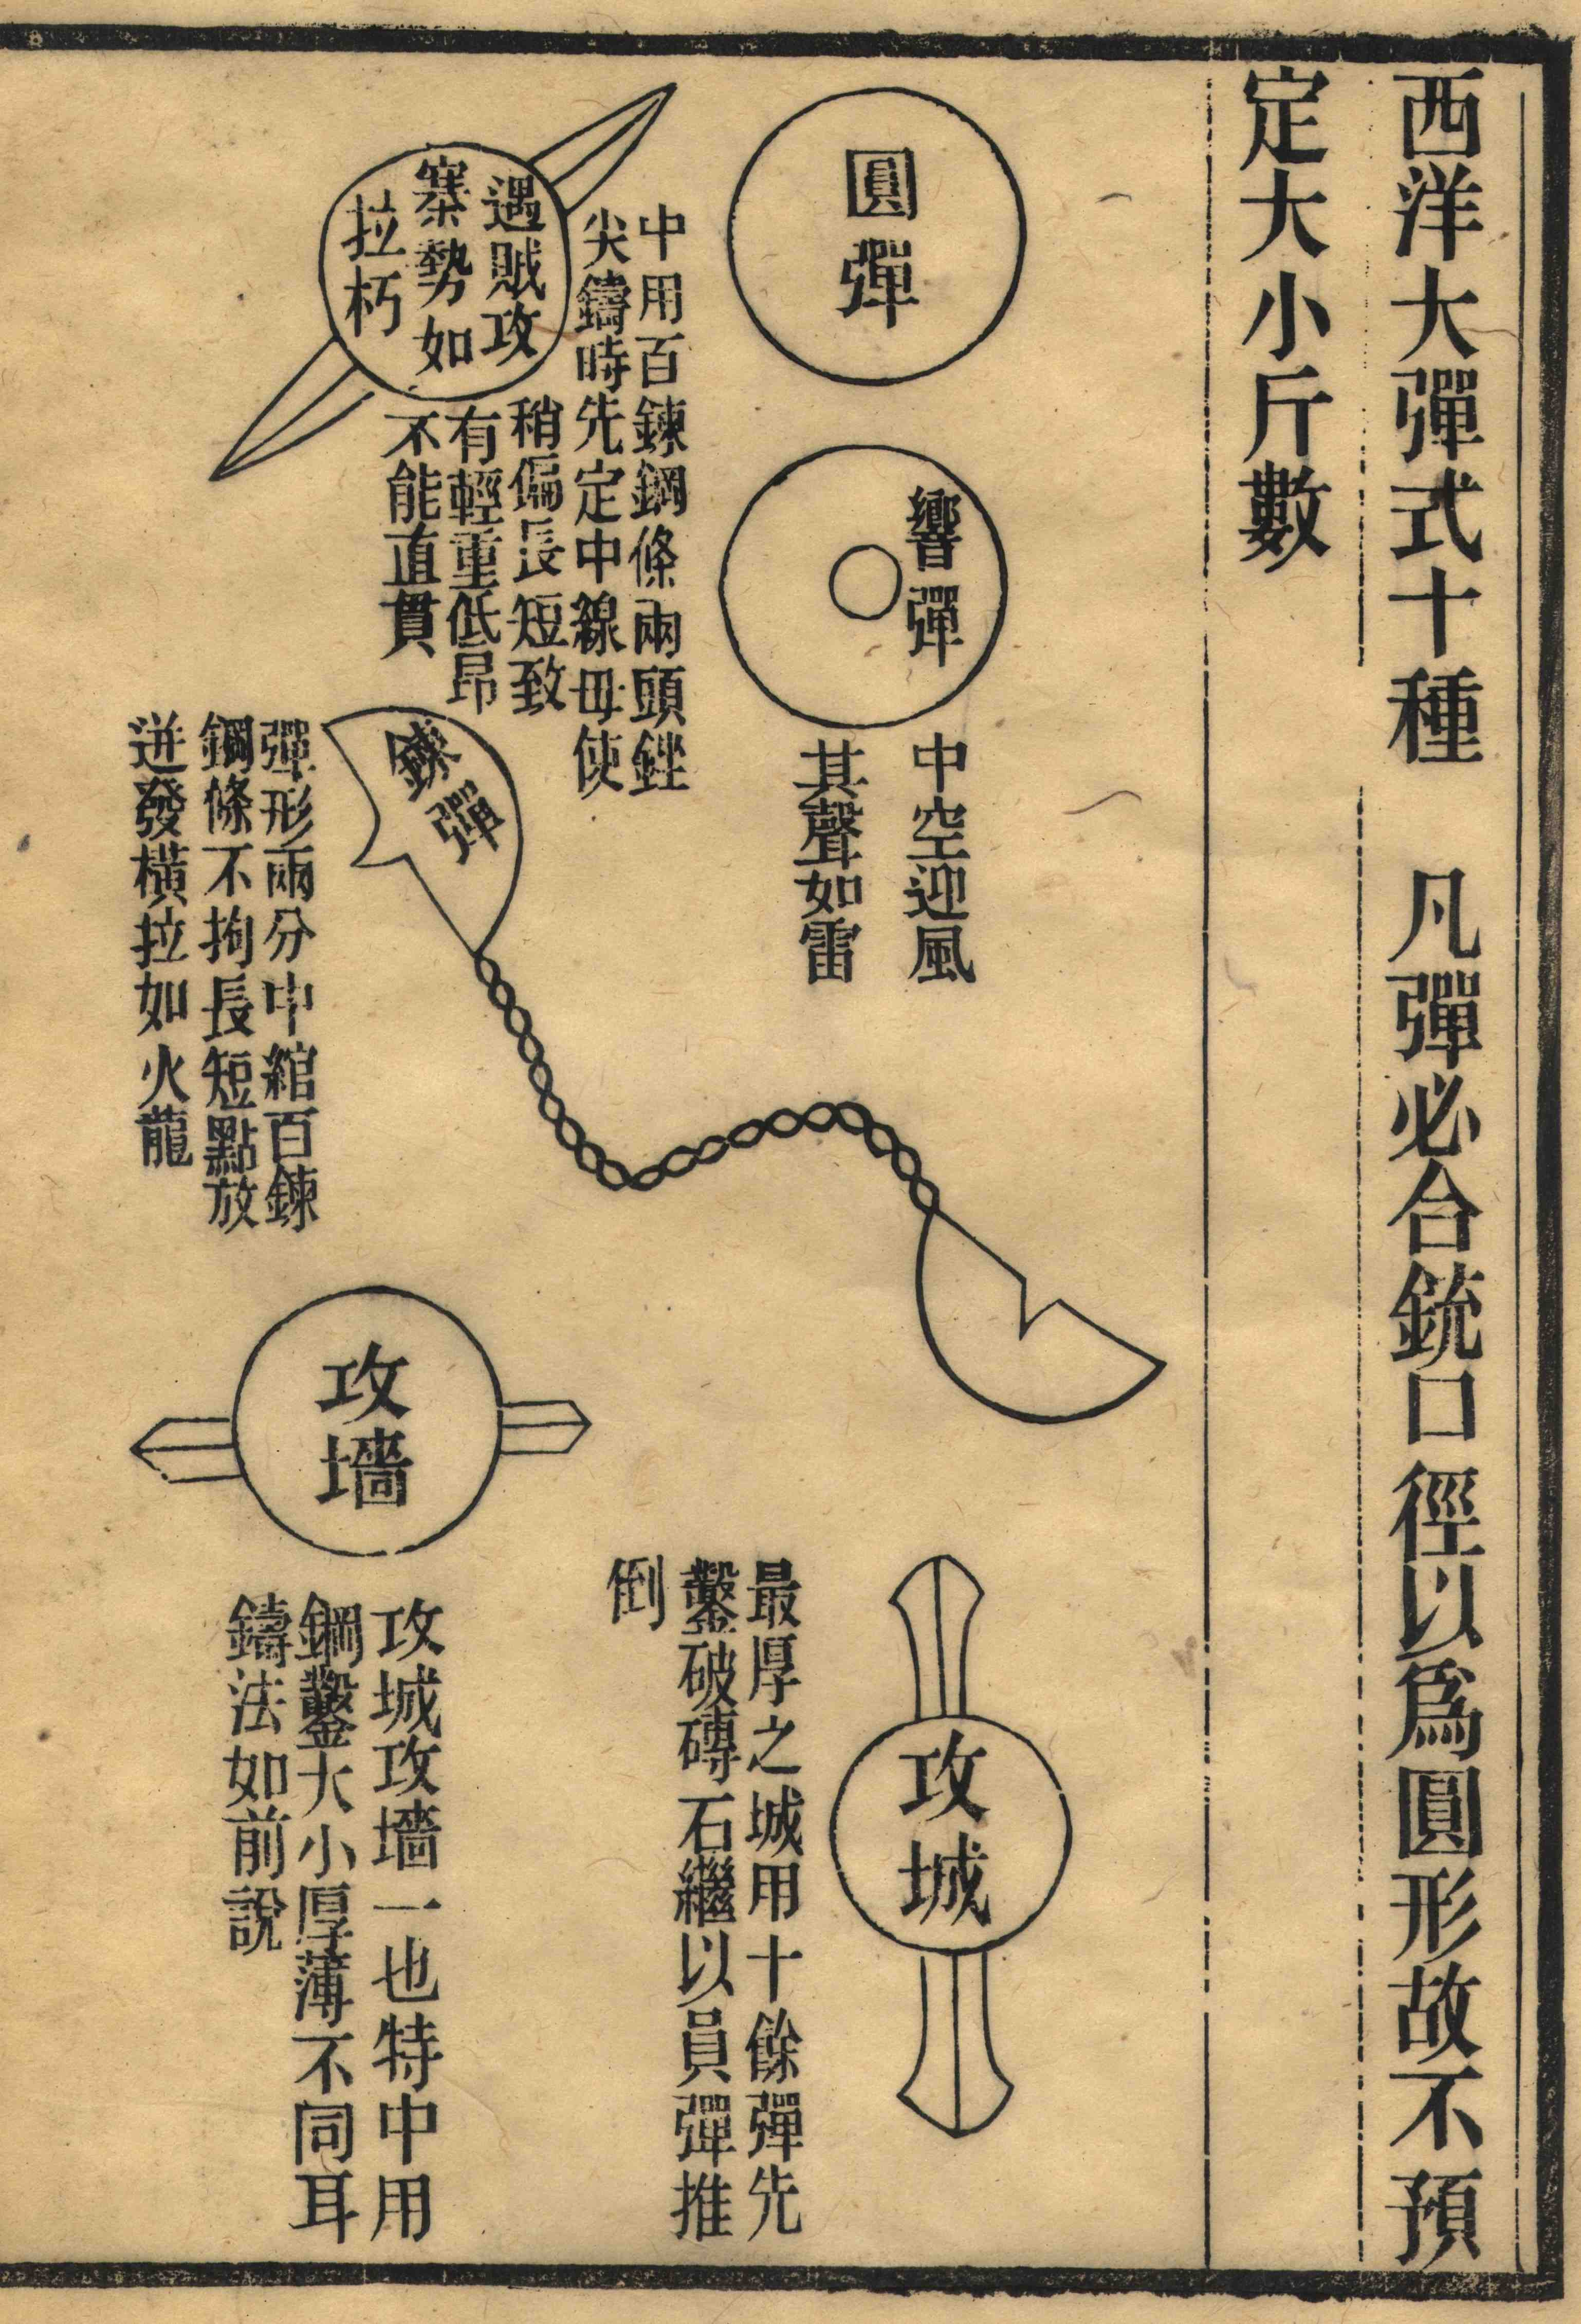
\includegraphics[height=12cm]{text16p69} \\
}
\end{tabular}

\begin{tabular}{@{}lll}
\parbox[b]{126.5mm}{
\begin{typeLatin}

\bold{<pb a><rh>}\chin{泰西事物起原 }\bold{<sm>}\chin{第三章}\bold{</sm></rh>} \\
\someText \\
\bold{<fig>} \\
\bold{<desc>}\chin{第二大派}\bold{</desc>} \\
\bold{<desc>}\chin{希伯流語}\bold{</desc>} \\
\bold{<desc>}\chin{亞刺比亞語}\bold{</desc>} \\ \\
\bold{<pb b><rh>}\chin{泰西事物起原 }\bold{<sm>}\chin{第三章}\bold{</sm></rh>} \\
\bold{<desc>}\chin{非尼西亞語}\bold{</desc>} \\
\someText \\[1mm]
\end{typeLatin}} & 
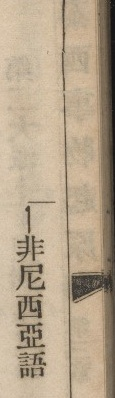
\includegraphics[height=5cm]{figure_14_33teil2} &
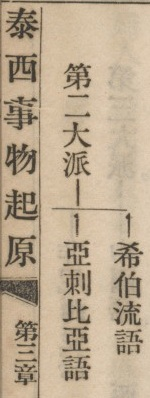
\includegraphics[height=5cm]{figure_14_33teil1}
\end{tabular}


\end{document}
